\documentclass[10pt,journal]{IEEEtran}

\usepackage{array}
\usepackage{booktabs}
\usepackage{cite}
\usepackage{graphicx}
\usepackage{xcolor}
\usepackage{amsmath}
\usepackage{amssymb}
\usepackage{tabularx}
\usepackage{makecell}
\usepackage{siunitx}
\usepackage{threeparttable}
\usepackage{listings}
\usepackage[most]{tcolorbox}
\usepackage{xparse}
\usepackage{url}
\urlstyle{tt}

\newcolumntype{Y}{>{\raggedright\arraybackslash}X}
\renewcommand{\arraystretch}{1.12}
\setlength{\tabcolsep}{3.5pt}
\sisetup{detect-weight=true,detect-family=true,round-mode=places,round-precision=3,table-number-alignment=center}

\definecolor{EchoGain}{RGB}{22,115,72}
\definecolor{EchoWarn}{RGB}{171,52,42}
\definecolor{EchoMuted}{RGB}{84,94,106}
\definecolor{CodeBg}{RGB}{248,250,252}
\definecolor{CodeFrame}{RGB}{203,213,225}
\definecolor{SrcHuman}{RGB}{235,246,255}
\definecolor{SrcGen}{RGB}{232,248,238}
\definecolor{SrcMixed}{RGB}{242,239,255}
\definecolor{SrcIP}{RGB}{255,242,204}
\newcommand{\kpigain}[1]{\textbf{\textcolor{EchoGain}{#1}}}
\newcommand{\kpicaveat}[1]{\textbf{\textcolor{EchoWarn}{#1}}}
\newcommand{\SrcKeyHuman}{\colorbox{SrcHuman}{\strut human-origin}}
\newcommand{\SrcKeyGen}{\colorbox{SrcGen}{\strut generated/evolved-origin}}
\newcommand{\SrcKeyMixed}{\colorbox{SrcMixed}{\strut mixed-origin}}
\newcommand{\SrcKeyIP}{\colorbox{SrcIP}{\strut redacted escrow-only}}
\newcommand{\SrcLineBase}[2]{\noindent\colorbox{#1}{\parbox{\dimexpr\linewidth-2\fboxsep}{\ttfamily\scriptsize #2}}\par}
\newcommand{\SrcLineHuman}[1]{\SrcLineBase{SrcHuman}{#1}}
\newcommand{\SrcLineGen}[1]{\SrcLineBase{SrcGen}{#1}}
\newcommand{\SrcLineMixed}[1]{\SrcLineBase{SrcMixed}{#1}}
\newcommand{\SrcLineIP}[1]{\SrcLineBase{SrcIP}{#1}}

\lstdefinestyle{EchoForgeCode}{
  basicstyle=\scriptsize\ttfamily,
  columns=fullflexible,
  breaklines=true,
  keepspaces=true,
  showstringspaces=false,
  frame=single,
  framerule=0.3pt,
  rulecolor=\color{CodeFrame},
  backgroundcolor=\color{CodeBg}
}
\newtcblisting{EchoCodeBox}[2][]{
  title={#2},
  listing only,
  listing options={style=EchoForgeCode,#1},
  colback=CodeBg,
  colframe=CodeFrame,
  coltitle=black,
  fonttitle=\bfseries\small,
  breakable
}

\graphicspath{{paper/figures/}{figures/}}

\begin{document}

\title{EchoForge: A Strict-Open Synthetic Benchmark for Low-Altitude UAS Radar and Multimodal Sensing}

\author{Jeppson Taylor, Lead Author\\
NeverHuman Research Group}

\maketitle

\begin{abstract}
EchoForge is a strict-open synthetic benchmark for low-altitude uncrewed aerial system (UAS) radar and multimodal sensing research. The paper-facing positive class is a fixed-wing pusher-prop public proxy with explicit uncertainty; it is not a measured-platform claim and is not a fielded-sensor surrogate. The final benchmark run contains 10,000 scenario groups, 50 positive groups, and 30,000 phase records. Candidate discovery, thresholding, and calibration use train/CV rows only; the blind group-locked holdout is scored once after selection lock. Primary KPI: LCB95 Recall@$\leq$1\%FPR. The accepted human-engineered prior fusion baseline is the comparator. On the 4,500-record blind holdout, with 24 positive records from eight positive scenario groups, Engineered Intelligence (EI) reaches point Recall@$\leq$1\%FPR of \kpigain{0.833 vs 0.292} (\kpigain{+54.2 pp}, \kpigain{+185.7\%}, \kpigain{2.85x}) and LCB95 Recall@$\leq$1\%FPR of \kpigain{0.713 vs 0.083} (\kpigain{+63.0 pp}, \kpigain{+760\%}, \kpigain{7.60x}). EI also raises average precision from \kpigain{0.128} to \kpigain{0.830} (\kpigain{+0.702}, about \kpigain{+547\%}) and cuts selected-threshold false positives from \kpigain{49 to 3} (\kpigain{93.9\% fewer false alarms}). \kpicaveat{EI ROC AUC is 0.916, below prior fusion's 0.938}, so the claim is improved low-FPR operating behavior for this synthetic public-proxy benchmark, not universal rank dominance. These results are reproducible benchmark evidence under declared assumptions, not measured truth, named-platform equivalence, or operational performance.
\end{abstract}

\begin{IEEEkeywords}
Synthetic radar, UAS detection, public proxy, micro-Doppler, sensor fusion, calibration, reproducibility, compare-only measured anchor.
\end{IEEEkeywords}

\section{Claim Boundary and Contributions}
EchoForge is intentionally narrower than a measured radar collection. It publishes public-proxy signatures and detector-facing products with explicit uncertainty and validation tiers, while keeping generated arrays, solver outputs, and measured raw files out of Git. The radar and detection framing follows standard signal-processing and CFAR practice rather than a sensor-surrogate claim \cite{skolnik2008,richards2014,rohling1983}. The paper-facing positive class is named \emph{fixed-wing pusher-prop public proxy}. No measured-platform truth, proprietary-equivalent behavior, fielded-system equivalence, or classified fidelity is claimed for any object, platform, or sensor.

The paper has one main experiment: compare accepted human-engineered radar/cue baselines and prior fusion against a locked EI sparse late-fusion artifact on the same blind, group-locked synthetic holdout. The contributions are:
\begin{itemize}
  \item a strict-open radar benchmark lane with explicit waveform, range-Doppler, clutter/noise/RFI, acoustic, passive-RF, and detector-view assumptions;
  \item a rare-positive, low-false-alarm evaluation protocol centered on LCB95 Recall@$\leq$1\%FPR, with AP, ROC AUC, calibration, and false-alarm families as guardrails;
  \item a detector/fusion benchmark that moves from human detectors to accepted prior fusion and then to EI under one split discipline;
  \item a generated evidence and source appendix that exposes model cards, CLI commands, source provenance, EI search traces, and no-holdout-selection guarantees.
\end{itemize}

\subsection{Core Experiment}
The core experiment compares classical radar and cue detector branches, tabular and sequence ML baselines, an accepted human-engineered prior fusion baseline, and EI sparse calibrated late fusion. Scenario groups are locked before phase expansion, train/CV rows are used for candidate discovery and calibration, and the blind holdout is scored once after selection lock. The claim tested is deliberately narrow: under the declared synthetic public-proxy generator and group-locked split, EI improves the low-FPR operating point over the accepted human-engineered prior fusion baseline. This comparator is not a straw baseline; it is the strongest non-EI late-fusion lane assembled from radar/cue branches under the same split and train/CV thresholding policy.

\begin{table*}[t]
  \caption{Core Experiment Roadmap}
  \label{tab:experimentroadmap}
  \centering
  \small
  \begin{tabular}{@{}p{0.18\textwidth}p{0.30\textwidth}p{0.23\textwidth}p{0.21\textwidth}@{}}
    \toprule
    Lane & What is modeled & Why it is in the paper & Reader-facing conclusion \\
    \midrule
    Sensor branches & X/Ku radar, S-band radar, GBAD cueing, acoustic cueing, and passive-RF provenance & Shows component evidence before fusion & Branches are sanity checks and failure-slice baselines \\
    Prior ML & Tabular and sequence learners trained only on detector-facing features & Tests ordinary learned controls under the same split & Useful controls, not the accepted-practice comparator \\
    Accepted fusion & Human-engineered layered fusion with train/CV thresholding & Represents accepted human-engineered prior fusion & Main comparator for EI \\
    EI sparse fusion & Train/CV candidate discovery, sparse nonnegative component fusion, monotone odds calibration, and one locked holdout pass & Tests whether EI improves the low-FPR operating point & Main challenger; claims are limited to this synthetic public-proxy benchmark \\
    \bottomrule
  \end{tabular}
\end{table*}

Benchmark positioning is compare-only. KTH provides a public 77~GHz FMCW measured anchor for drone/bird/human observable-shape checks; Open Radar and RAD-DAR/RDRD provide public radar and range-Doppler reference points; and public UAS micro-Doppler studies bound the observable families used for small aerial objects \cite{kth2021,openradar2023,raddar2019,han2026,rahman2018,molchanov2014,ritchie2017}. EchoForge does not replace those measured collections. It provides a strict-open synthetic lane for controlled hard negatives, leakage checks, and low-FPR detector comparison when measured positive-class truth is not available.

\begin{figure*}[t]
  \centering
  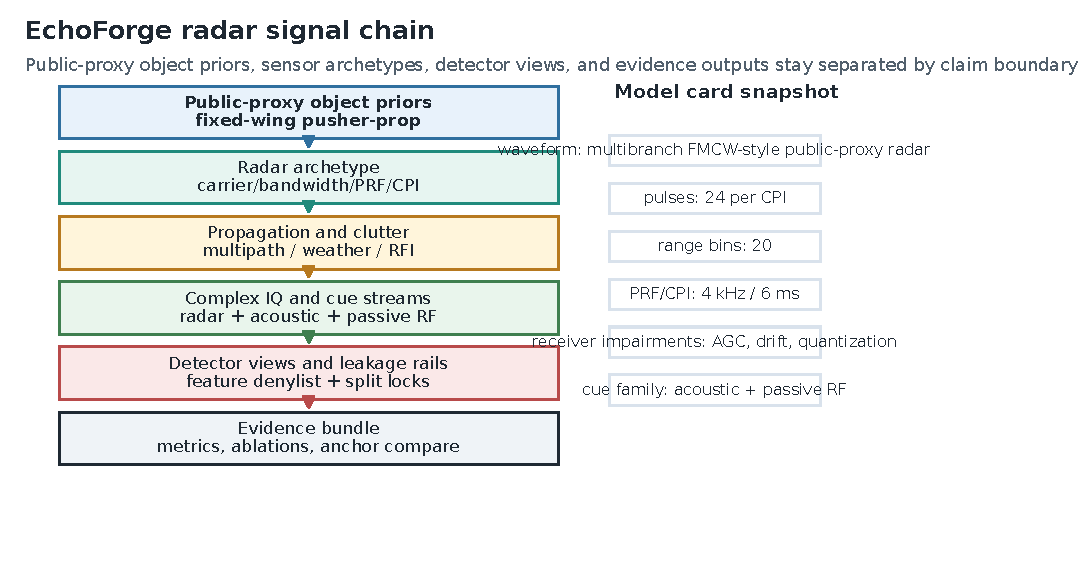
\includegraphics[width=0.96\textwidth]{architecture_stack.pdf}
  \caption{Radar signal chain and claim boundary. Public-proxy object priors, radar archetype assumptions, clutter and artifact priors, detector views, and evidence outputs are separated so the benchmark can be audited without conflating synthetic products with measured truth.}
  \label{fig:architecture}
\end{figure*}

\section{Data Processing and Evidence Flow}
EchoForge should be read as a pipeline, not as a ledger of disconnected artifacts. Figure~\ref{fig:dataprocessing} is the reviewer-facing trace: scenario groups are sampled, expanded into phase records, converted into synthetic radar/cue products, materialized as detector-view features through a denylisted schema, searched/calibrated on train/CV rows, locked, and scored once on blind holdout. The paper evidence manifest is labeled \texttt{tier1-final}, and the key generated rows are \texttt{data\_processing\_trace\_rows.csv}, \texttt{simulation\_best\_practice\_rows.csv}, \texttt{phase\_method\_ladder\_rows.csv}, \texttt{ei\_evolution\_trace.csv}, and \texttt{source\_appendix\_hashes.csv}.

\begin{figure*}[t]
  \centering
  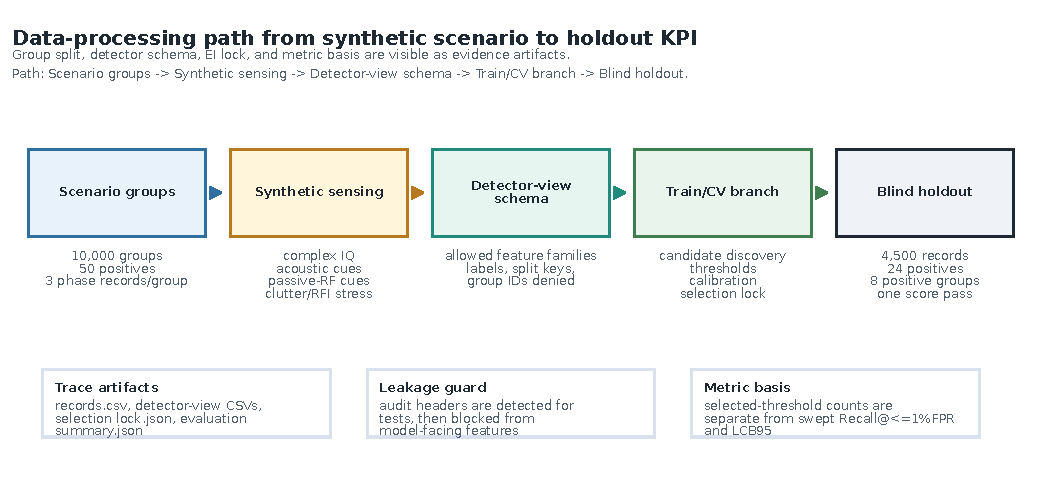
\includegraphics[width=0.98\textwidth]{data_processing_flow.pdf}
  \caption{End-to-end data-processing path. Scenario groups and phase records generate synthetic radar/cue products; detector-view materialization enforces feature denylisting; train/CV rows drive candidate discovery, thresholds, and monotone calibration; and the blind holdout is scored once after selection lock.}
  \label{fig:dataprocessing}
\end{figure*}

\begin{table*}[t]
  \caption{Data Processing Traceability Checklist}
  \label{tab:dataprocessing}
  \centering
  \small
  \begin{tabular}{@{}p{0.18\textwidth}p{0.24\textwidth}p{0.26\textwidth}p{0.22\textwidth}@{}}
    \toprule
    Stage & Produced artifact & Reviewer check & Failure mode guarded \\
    \midrule
    Scenario sampling & \texttt{scenario\_manifest.csv}, \texttt{dataset\_manifest.json} & group IDs and split roles exist before phase expansion & row-level leakage through repeated phases \\
    Synthetic sensing & \texttt{records.csv}, raw IQ references, acoustic and passive-RF cue summaries & generated radar/cue products inherit public-proxy priors and group split & undocumented signal-source mixing \\
    Detector views & detector-view CSVs and \texttt{detector\_view\_schema\_evidence.csv} & labels, group IDs, split keys, audit headers, and generator metadata are blocked & shortcut learning from audit fields \\
    Train/CV branch & \texttt{selection\_lock.json}, component weights, thresholds, calibrators & candidate search, weighting, thresholding, and calibration are train/CV-only & holdout tuning or silent reselection \\
    Blind holdout & \texttt{evaluation\_summary.json}, \texttt{main\_kpi\_gain\_table.csv} & selected-threshold counts, swept Recall@$\leq$1\%FPR, and LCB95 are separate fields & conflating locked-threshold counts with swept low-FPR recall \\
    \bottomrule
  \end{tabular}
\end{table*}

\section{Simulation and Monte Carlo}
EchoForge uses a clean-room signal-chain proxy rather than a proprietary sensor surrogate. The received-power proxy is
\begin{equation}
P_r \propto \frac{P_t G_t G_r \lambda^2 \sigma(\theta, f, \phi)}{(4\pi)^3 R^4 L},
\end{equation}
where $\sigma$ is an aspect- and frequency-dependent public-proxy RCS term, $R$ is slant range, and $L$ is aggregate loss. Complex IQ is generated as a phase-stable target term plus clutter, interference, and receiver impairment terms,
\begin{equation}
x_{m,n} = a_{m,n} e^{j(2\pi f_d mT_r + \varphi_n)} + c_{m,n} + \epsilon_{m,n}.
\end{equation}
The benchmark keeps these values synthetic: absolute scale is a proxy, and object priors are public-source envelopes rather than measured signatures \cite{chen2011,tahmoush2015,rahman2018,ezuma2019,molchanov2014,ritchie2017}.

\subsection{Radar Simulation Best Practices}
The simulation follows standard radar-review practice while keeping the claim boundary explicit. Waveform assumptions expose carrier frequency, bandwidth, CPI, PRF/CRF, pulse/chirp count, range span, range resolution, Doppler resolution, and velocity resolution. The range-Doppler proxy uses
\begin{equation}
\Delta R = \frac{c}{2B}, \qquad \Delta f_D = \frac{1}{T_{\mathrm{CPI}}}, \qquad \Delta v = \frac{\lambda}{2T_{\mathrm{CPI}}},
\end{equation}
with approximate unambiguous velocity $\lambda f_{\mathrm{PRF}}/4$ for branch cards. Public-proxy target modeling includes fixed-wing pusher-prop geometry, aspect RCS uncertainty, Swerling-like fluctuation, scenario kinematics, and a broad 150--217~Hz pusher-prop micro-Doppler prior. Hard negatives include birds and RC fixed-wing with overlapping cadence or aspect. Environment and receiver stress include Weibull/K-like clutter, thermal noise buckets, phase noise, AGC compression, ADC quantization, dropped CPI, Doppler folding, calibration offset, RFI bursts, and multipath masking \cite{ward1990,kay1998,vantrees2002,swerling1954}.

\begin{table*}[t]
  \caption{Radar Model Card and Derived Resolution Assumptions}
  \label{tab:radar}
  \centering
  \small
  \begin{tabular}{@{}lrrrrrrrr@{}}
    \toprule
    Branch & $f_0$ GHz & BW MHz & PRF/CRF Hz & CPI ms & Chirps & Span m & $\Delta R$ m & $\Delta v$ m/s \\
    \midrule
    X/Ku C-UAS & 10.0 & 600 & 4000/4000 & 6.0 & 24 & 5.0 & 0.250 & 2.498 \\
    S-band AESA/MHR & 3.1 & 180 & 4000/4000 & 6.0 & 24 & 16.7 & 0.833 & 8.059 \\
    GBAD 3D/4D & 10.3 & 300 & 4000/4000 & 6.0 & 24 & 10.0 & 0.500 & 2.426 \\
    \bottomrule
  \end{tabular}
\end{table*}

\subsection{Monte Carlo Scenario Construction}
The main run consists of 10,000 scenario groups, 50 positive groups, and 30,000 phase records generated from one seed. Each group receives site, range, aspect, weather/noise, hard-negative family, and positive/negative role, then expands into three locked windows: initial take-up, climb transition, and cruise altitude. Split assignment occurs at the scenario-group level so all phase records from one group share the same split role and fold. The final holdout contains 1,500 groups with eight positive groups and 24 positive phase records; the train/CV branch contains the remaining 42 positive groups. The evidence bundle emits \texttt{monte\_carlo\_setup\_rows.csv} to make the randomization and group lock inspectable.

\begin{figure*}[t]
  \centering
  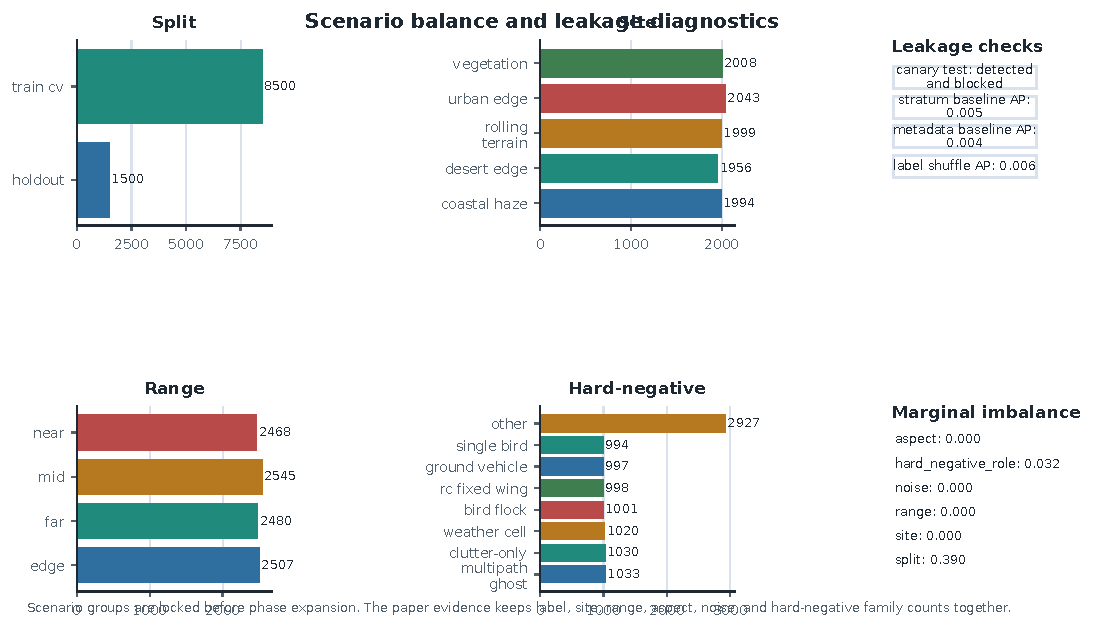
\includegraphics[width=0.98\textwidth]{monte_carlo_split_flow.pdf}
  \caption{Scenario balance and leakage diagnostics. Scenario groups are locked before phase expansion, and the evidence bundle keeps split, label, site, range, aspect, noise, and hard-negative family counts together with canary and sanity checks. Audit-only split/group headers are reported as detected and blocked by the model-facing schema rather than as detector features.}
  \label{fig:splitflow}
\end{figure*}

\section{Detector Views and Human Baselines}
The raw data product is a synthetic intermediate: raw IQ references, range-Doppler diagnostics, acoustic cue summaries, passive-RF cue summaries, and scenario records. The detector-processing contract reduces those products to branch-level views. Model-facing matrices receive score summaries and cue features; labels, split keys, group IDs, audit headers, time locks, and restricted generator state are blocked by the feature denylist. This is the Detector-View Modeling Contract carried by \texttt{detector\_view\_schema\_evidence.csv}.

\begin{table*}[t]
  \caption{Detector-Processing Baseline Ladder}
  \label{tab:detectorbaseline}
  \centering
  \small
  \begin{tabular}{@{}p{0.19\textwidth}p{0.34\textwidth}p{0.35\textwidth}@{}}
    \toprule
    Lane & Processing idea & Role in comparison \\
    \midrule
    X/Ku radar & CFAR-style range-Doppler concentration, micro-Doppler spread, clutter stress & High-resolution radar branch sanity check \cite{rohling1983,richards2014,kay1998} \\
    S-band radar & Coarser MTD/range-velocity summaries and track confidence & Tactical radar branch stress check \cite{schleher1999,richards2014,vantrees2002} \\
    GBAD cueing & Horizon/revisit/stale-track cue score & Wide-area cueing branch check \\
    Acoustic cue & Spectral cadence, amplitude stability, node agreement & Propulsion-cadence supporting cue \\
    Passive RF & No-signal, RFI burst, provenance quality, sparse RF cue geometry & Missingness and multimodal provenance stress \\
    Prior ML & Tabular and sequence learners on denylisted detector views & Ordinary learned controls under the same split \\
    Accepted fusion & Human-engineered layered fusion with train/CV thresholding & Main accepted-practice comparator for EI \\
    \bottomrule
  \end{tabular}
\end{table*}

Detector archetypes are public-source role envelopes. The X/Ku C-UAS branch is anchored by public descriptions of low-slow-small radar behavior such as Blighter A400 and KuRFS \cite{blighterA400,rtxKurfs}. The tactical S-band branch follows public MHR/nMHR-style hemispheric surveillance roles \cite{drsRadaNmhr}. The GBAD cueing branch follows public wide-area 3D/4D radar roles such as Giraffe 1X and Sentinel summaries \cite{saabGiraffe1X,rtxSentinel}. Public role envelope means plausible branch role and observable family, not sensitivity, ECCM, exact Pd/Pfa, or military performance.

\section{Sensor Fusion Baseline}
Low-altitude UAS detection is rarely a single-detector problem. Radar branches see range-Doppler and track structure; acoustic cues see cadence and cross-node agreement; passive-RF cues see absence, contamination, and provenance. Classical multisensor fusion, tracking/data association, and multi-source uncertainty practice motivate an accepted fusion comparator before EI is introduced \cite{hall1997,barshalom2001,blackman1999,mahler2007}. The accepted prior fusion lane combines branch evidence while preserving human-designed thresholding and calibration. EI is judged against this fusion lane, not against a deliberately weak single detector.

\begin{figure*}[t]
  \centering
  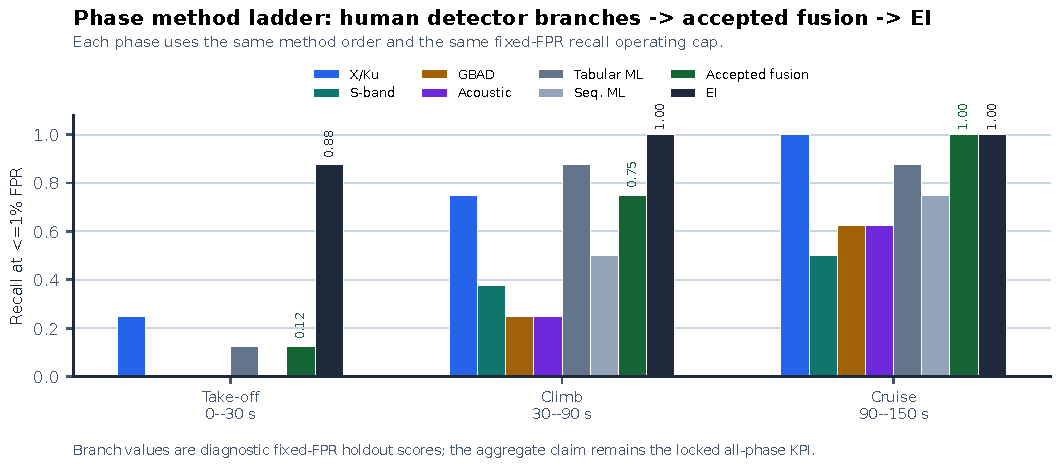
\includegraphics[width=0.98\textwidth]{phase_method_ladder.pdf}
  \caption{Phase-wise method ladder. The same three scenario panels show progression from human detector branches to accepted fusion and then to EI. The plotted operating metric is Recall@$\leq$1\%FPR when available, with AP retained as a secondary diagnostic for branch rows.}
  \label{fig:phasemethodladder}
\end{figure*}

\section{Engineered Intelligence}
EI is implemented as auditable algorithm discovery rather than as an opaque model handle. It decomposes the problem into candidate score families, evolves and ranks sparse nonnegative combinations on train/CV rows, fits a monotone odds calibrator, writes a selection lock, and then scores holdout once. The source is observable; the evidence bundle records source hashes, component weights, trace rows, and the no-holdout-selection policy. This framing is aligned with program-search and agentic scientific-discovery work, while keeping the benchmark claim narrow and reproducible \cite{funsearch2024,aiScientist2024,aiScientistV22025,alphaEvolve2025}.

\begin{table}[t]
  \caption{EI Candidate Discovery and Locked Scoring Algorithm}
  \label{tab:eialgorithm}
  \centering
  \small
  \begin{tabular}{@{}p{0.12\columnwidth}p{0.77\columnwidth}@{}}
    \toprule
    Step & Operation \\
    \midrule
    1 & Read train/CV detector-view scores after the denylist removes labels, split fields, group IDs, time locks, and audit headers. \\
    2 & Generate candidate component families from radar, passive-RF, acoustic, transport/geometry, and fusion-context score views. \\
    3 & Optimize sparse nonnegative component weights on train/CV rows only. \\
    4 & Fit a monotone geodesic-odds calibrator and threshold policy without holdout rows. \\
    5 & Write \texttt{selection\_lock.json} and freeze component IDs, weights, calibrator, and threshold source. \\
    6 & Score the blind holdout once and emit KPI, calibration, false-alarm, and leakage evidence. \\
    \bottomrule
  \end{tabular}
\end{table}

\begin{figure*}[t]
  \centering
  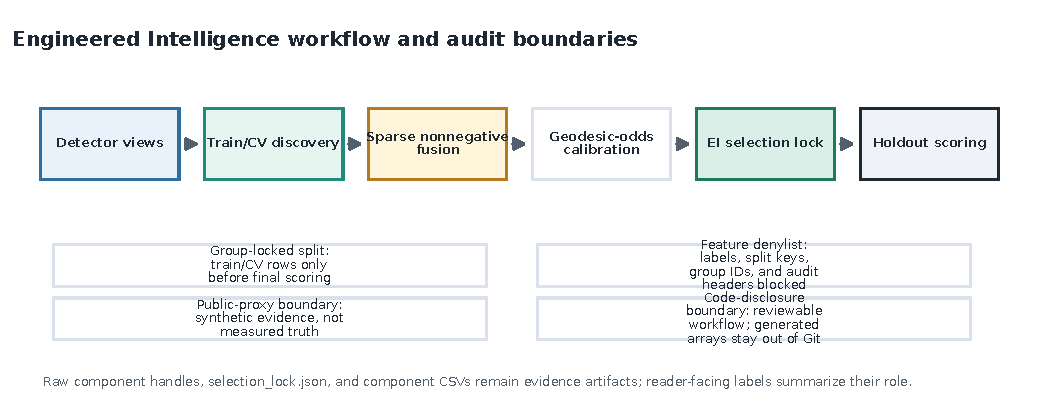
\includegraphics[width=0.98\textwidth]{ei_workflow.pdf}
  \caption{Engineered Intelligence workflow and audit boundaries. Detector-view tables, train/CV-only candidate discovery, sparse nonnegative fusion, geodesic-odds calibration, EI selection lock, and blind holdout scoring are separated from group-lock, feature-denylist, claim-boundary, and code-disclosure rails.}
  \label{fig:eiworkflow}
\end{figure*}

\subsection{Evolution Trace and Locked Holdout Endpoint}
The most important EI audit artifact is the search trace, not only the final score. The advanced lane writes \texttt{evolution\_trace.csv} with candidate order, stage, family, calibrator, feature/component count, train/CV objective, train/CV AP, train/CV ROC AUC, running-best values, and exactly one CV-chosen row. The paper evidence normalizer emits \texttt{ei\_evolution\_trace.csv} and \texttt{ei\_evolution\_summary.json}. Every trace row has \texttt{selection\_split=train\_cv} and \texttt{holdout\_rows\_used\_for\_selection=0}.

This separation is essential. A curve of holdout scores across candidate attempts would invite holdout shopping unless each point came from a separately pre-declared lock. EchoForge therefore reports the search trajectory as train/CV evidence and shows the holdout only once, as the endpoint of \texttt{selection\_lock.json}. The holdout is not used to draw the evolution curve.

\begin{figure*}[t]
  \centering
  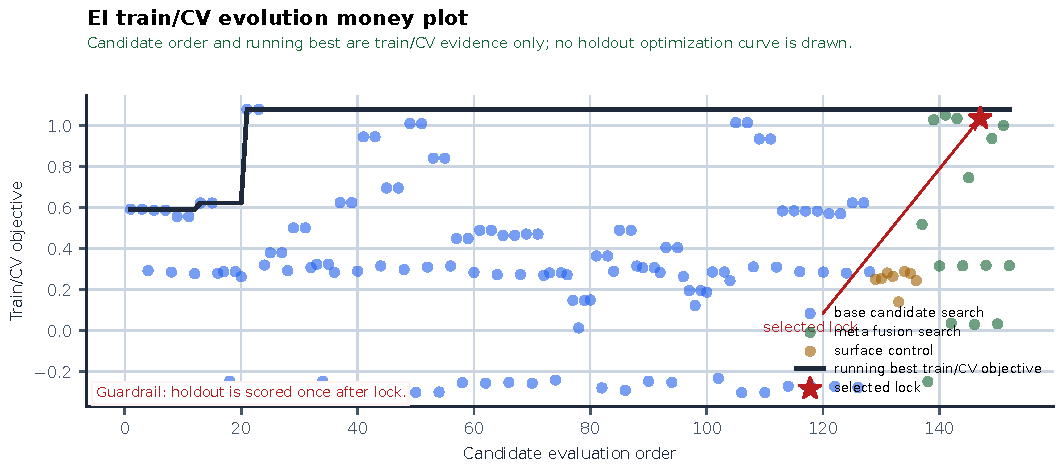
\includegraphics[width=0.98\textwidth]{ei_evolution_money_plot.pdf}
  \caption{EI evolution money plot. Left: internal train/CV candidate evaluations in actual evaluation order with the running best shown as a bold line. Middle: best train/CV AP reached by each search stage. Right: the single locked holdout endpoint after the selection lock. The holdout is not used to draw the evolution curve.}
  \label{fig:eievolution}
\end{figure*}

\begin{table*}[t]
  \caption{EI Evolution Trace Audit Contract}
  \label{tab:eievolutioncontract}
  \centering
  \small
  \begin{tabular}{@{}p{0.18\textwidth}p{0.30\textwidth}p{0.24\textwidth}p{0.20\textwidth}@{}}
    \toprule
    Artifact & Required fields & Reviewer check & Failure mode guarded \\
    \midrule
    \texttt{evolution\_trace.csv} & candidate order, stage, family, calibrator, train/CV metrics, running best & actual search trace rather than sorted leaderboard & fake evolution plot \\
    \texttt{selection\_lock.json} & frozen component IDs, weights, calibrator, threshold source, no-holdout policy & trace row matches the locked artifact & silent reselection \\
    \texttt{ei\_evolution\_summary.json} & trace basis, selected row, one holdout endpoint & strict mode fails on leaderboard-only fallback & rank-order masquerading as evolution \\
    Holdout endpoint & AP, ROC AUC, FPR, F1, gate status for the locked artifact only & holdout appears once after lock & holdout tuning \\
    \bottomrule
  \end{tabular}
\end{table*}

\section{Evaluation Protocol}
Let $s_i$ be a detector score. For EI, the fused score is a nonnegative weighted sum over component scores,
\begin{equation}
z_i = \sum_{j=1}^{k} w_j s_{ij}, \qquad w_j \ge 0, \qquad \sum_{j=1}^{k} w_j = 1.
\end{equation}
The paper-facing calibration step is a monotone geodesic-odds transform,
\begin{equation}
\hat p_i = \sigma\!\left(a \log \frac{z_i + \epsilon}{1 - z_i + \epsilon} + b\right),
\end{equation}
where $\sigma$ is the logistic function. Thresholds and calibrators are fit on train/CV rows only. The evaluation metrics are ROC AUC, AP, Recall@$\leq$1\%FPR, accuracy, precision, recall, FPR, F1, Brier score, and ECE. Group-block bootstrap confidence intervals resample scenario groups, not phase rows, which matches the locked group structure \cite{fishman1996,metropolis1953,rubinstein2016,kohavi1995}. Calibration and classifier diagnostics follow standard practice \cite{fawcett2006,davis2006,saito2015,platt1999,niculescu2005,guo2017,bishop2006,hastie2009,pedregosa2011}.

\subsection{Primary KPI}
The headline KPI is the lower 95\% group-block bootstrap bound of recall at FPR $\leq 1\%$, abbreviated LCB95 Recall@$\leq$1\%FPR. AP, ROC AUC, raw recall, precision, F1, calibration, and false-alarm breakdowns are guardrails. Three quantities are kept separate: selected-threshold TP/FP/FN counts use the threshold fixed by train/CV or the EI lock; Recall@$\leq$1\%FPR is a swept holdout operating-point diagnostic; and LCB95 is the 2.5th percentile of the group-block bootstrap distribution for that swept low-FPR recall.

\section{Results}
\begin{table}[t]
  \caption{Main KPI Gain Ledger Versus Accepted Prior Fusion}
  \label{tab:mainkpigain}
  \centering
  \small
  \begin{tabular}{@{}p{0.34\columnwidth}rrp{0.22\columnwidth}@{}}
    \toprule
    Metric & Prior & EI & Change \\
    \midrule
    LCB95 Recall@$\leq$1\%FPR & 0.083 & \kpigain{0.713} & \kpigain{+760\%, 7.60x} \\
    Point Recall@$\leq$1\%FPR & 0.292 & \kpigain{0.833} & \kpigain{+185.7\%, 2.85x} \\
    Average precision & 0.128 & \kpigain{0.830} & \kpigain{about +547\%} \\
    Selected-threshold FP & 49 & \kpigain{3} & \kpigain{93.9\% fewer} \\
    F1 & 0.241 & \kpigain{0.826} & \kpigain{+243\%} \\
    ROC AUC & 0.938 & \kpicaveat{0.916} & \kpicaveat{guardrail trade-off} \\
    \bottomrule
  \end{tabular}
\end{table}

\begin{figure*}[t]
  \centering
  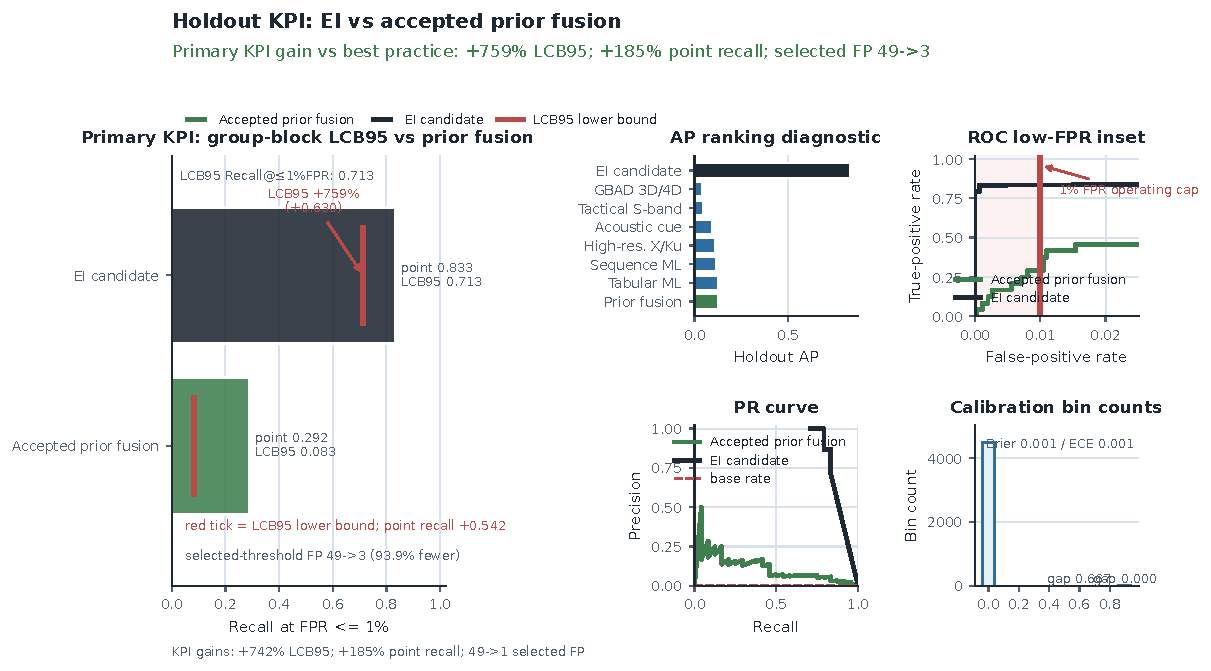
\includegraphics[width=0.98\textwidth]{kpi_ranking.pdf}
  \caption{Holdout primary KPI, ranking diagnostics, low-FPR ROC/PR behavior, and calibration. Red vertical ticks are group-block LCB95 lower bounds, and the pale red shaded zone with the thick red line marks the 1\% FPR operating cap. Recall@$\leq$1\%FPR and its LCB95 are the headline quantities; AP, ROC AUC, PR shape, and calibration bins are supporting diagnostics.}
  \label{fig:kpi}
\end{figure*}

\begin{table*}[t]
  \caption{Holdout Summary Separating Ranking, Selected-Threshold Counts, and Swept Fixed-FPR Metrics}
  \label{tab:metrics}
  \centering
  \small
  \begin{tabular}{@{}lrrrrlrrrr@{}}
    \toprule
    Method & AP & ROC AUC & F1 & ECE & Threshold source & TP/FP/FN & Sel. FPR & Recall@$\leq$1\%FPR & LCB95 \\
    \midrule
    accepted prior fusion & 0.128 & 0.938 & 0.241 & 0.016 & train/CV max-F1 & 10/49/14 & 0.010947 & 0.292 & 0.083 \\
    EI & 0.830 & 0.916 & 0.826 & 0.002 & EI selection lock & 19/3/5 & 0.000670 & 0.833 & 0.713 \\
    EI gain vs prior & +0.702 & -0.021 & +0.585 & -0.014 & locked vs train/CV & +9/-46/-9 & -0.010277 & +0.542 & +0.630 \\
    \bottomrule
  \end{tabular}
\end{table*}

\begin{figure*}[t]
  \centering
  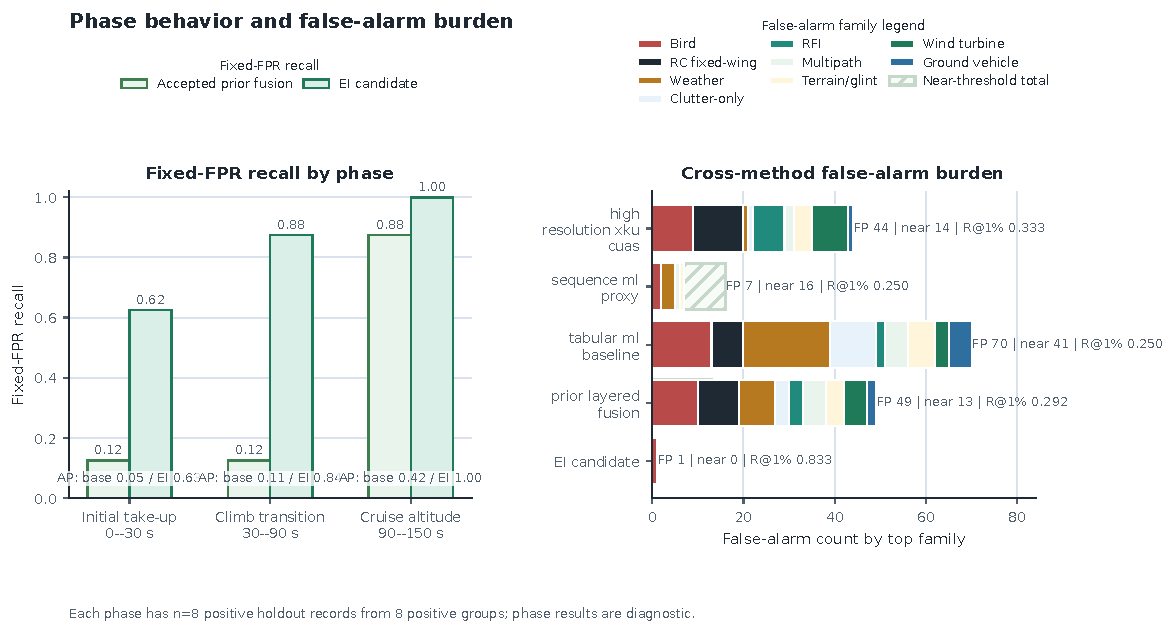
\includegraphics[width=0.98\textwidth]{phase_kpi.pdf}
  \caption{Per-phase fixed-FPR recall and cross-method false-positive burden. The left panel keeps the operating metric simple: bars are Recall@$\leq$1\%FPR for accepted prior fusion and EI, while AP is printed only as diagnostic text. The right-panel false-alarm family legend maps stacked colors to hard-negative families; pale/hatched bars show near-threshold totals, and the FP, near, and R@1\% labels are diagnostic robustness context. Each phase has only eight positive holdout records from eight positive groups, so phase conclusions are diagnostic.}
  \label{fig:phasekpi}
\end{figure*}

The gain row is the direct result: EI raises the primary LCB95 metric by +0.630, raises point Recall@$\leq$1\%FPR by +0.542, and reduces selected-threshold false positives from 49 to 3 while conceding ROC AUC. Because the positive holdout has $n=8$ groups, phase and family conclusions are diagnostic rather than stable field-rate estimates.

\section{Diagnostics}
\begin{figure*}[t]
  \centering
  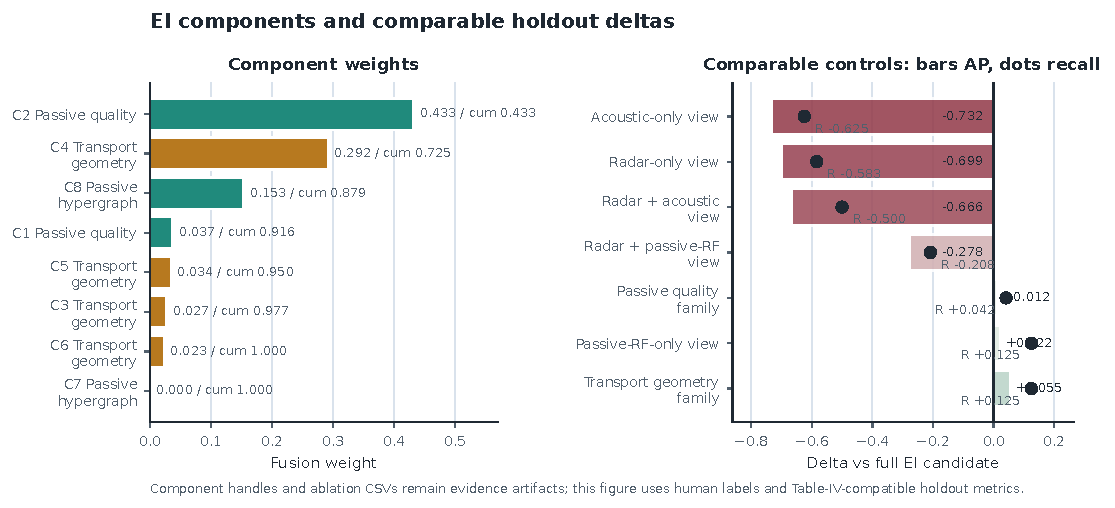
\includegraphics[width=0.98\textwidth]{detector_ml_pipeline.pdf}
  \caption{EI component weights and comparable holdout controls. The left panel sorts human-readable component weights; the right panel reports AP and fixed-FPR recall deltas computed with the same main holdout-table-compatible metric definitions as Table~\ref{tab:metrics}. Raw component handles and ablation-internal diagnostics remain in evidence artifacts.}
  \label{fig:ablation}
\end{figure*}

\begin{figure*}[t]
  \centering
  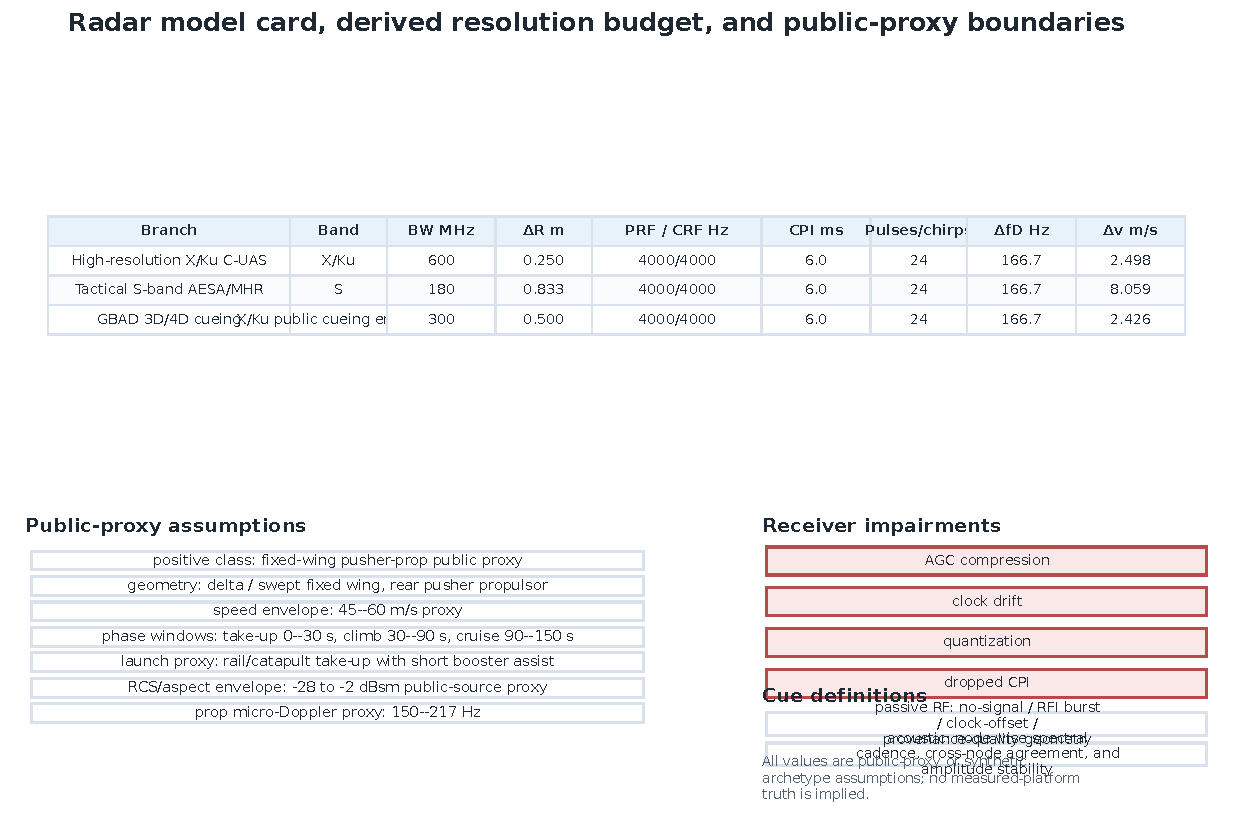
\includegraphics[width=0.98\textwidth]{iq_drone_samples.pdf}
  \caption{Radar model card and signal-chain parameter panel. The figure surfaces the public-proxy assumptions behind the benchmark so detector results can be read against explicit carrier, bandwidth, PRF/CPI, and cue definitions.}
  \label{fig:radarcard}
\end{figure*}

\begin{figure*}[t]
  \centering
  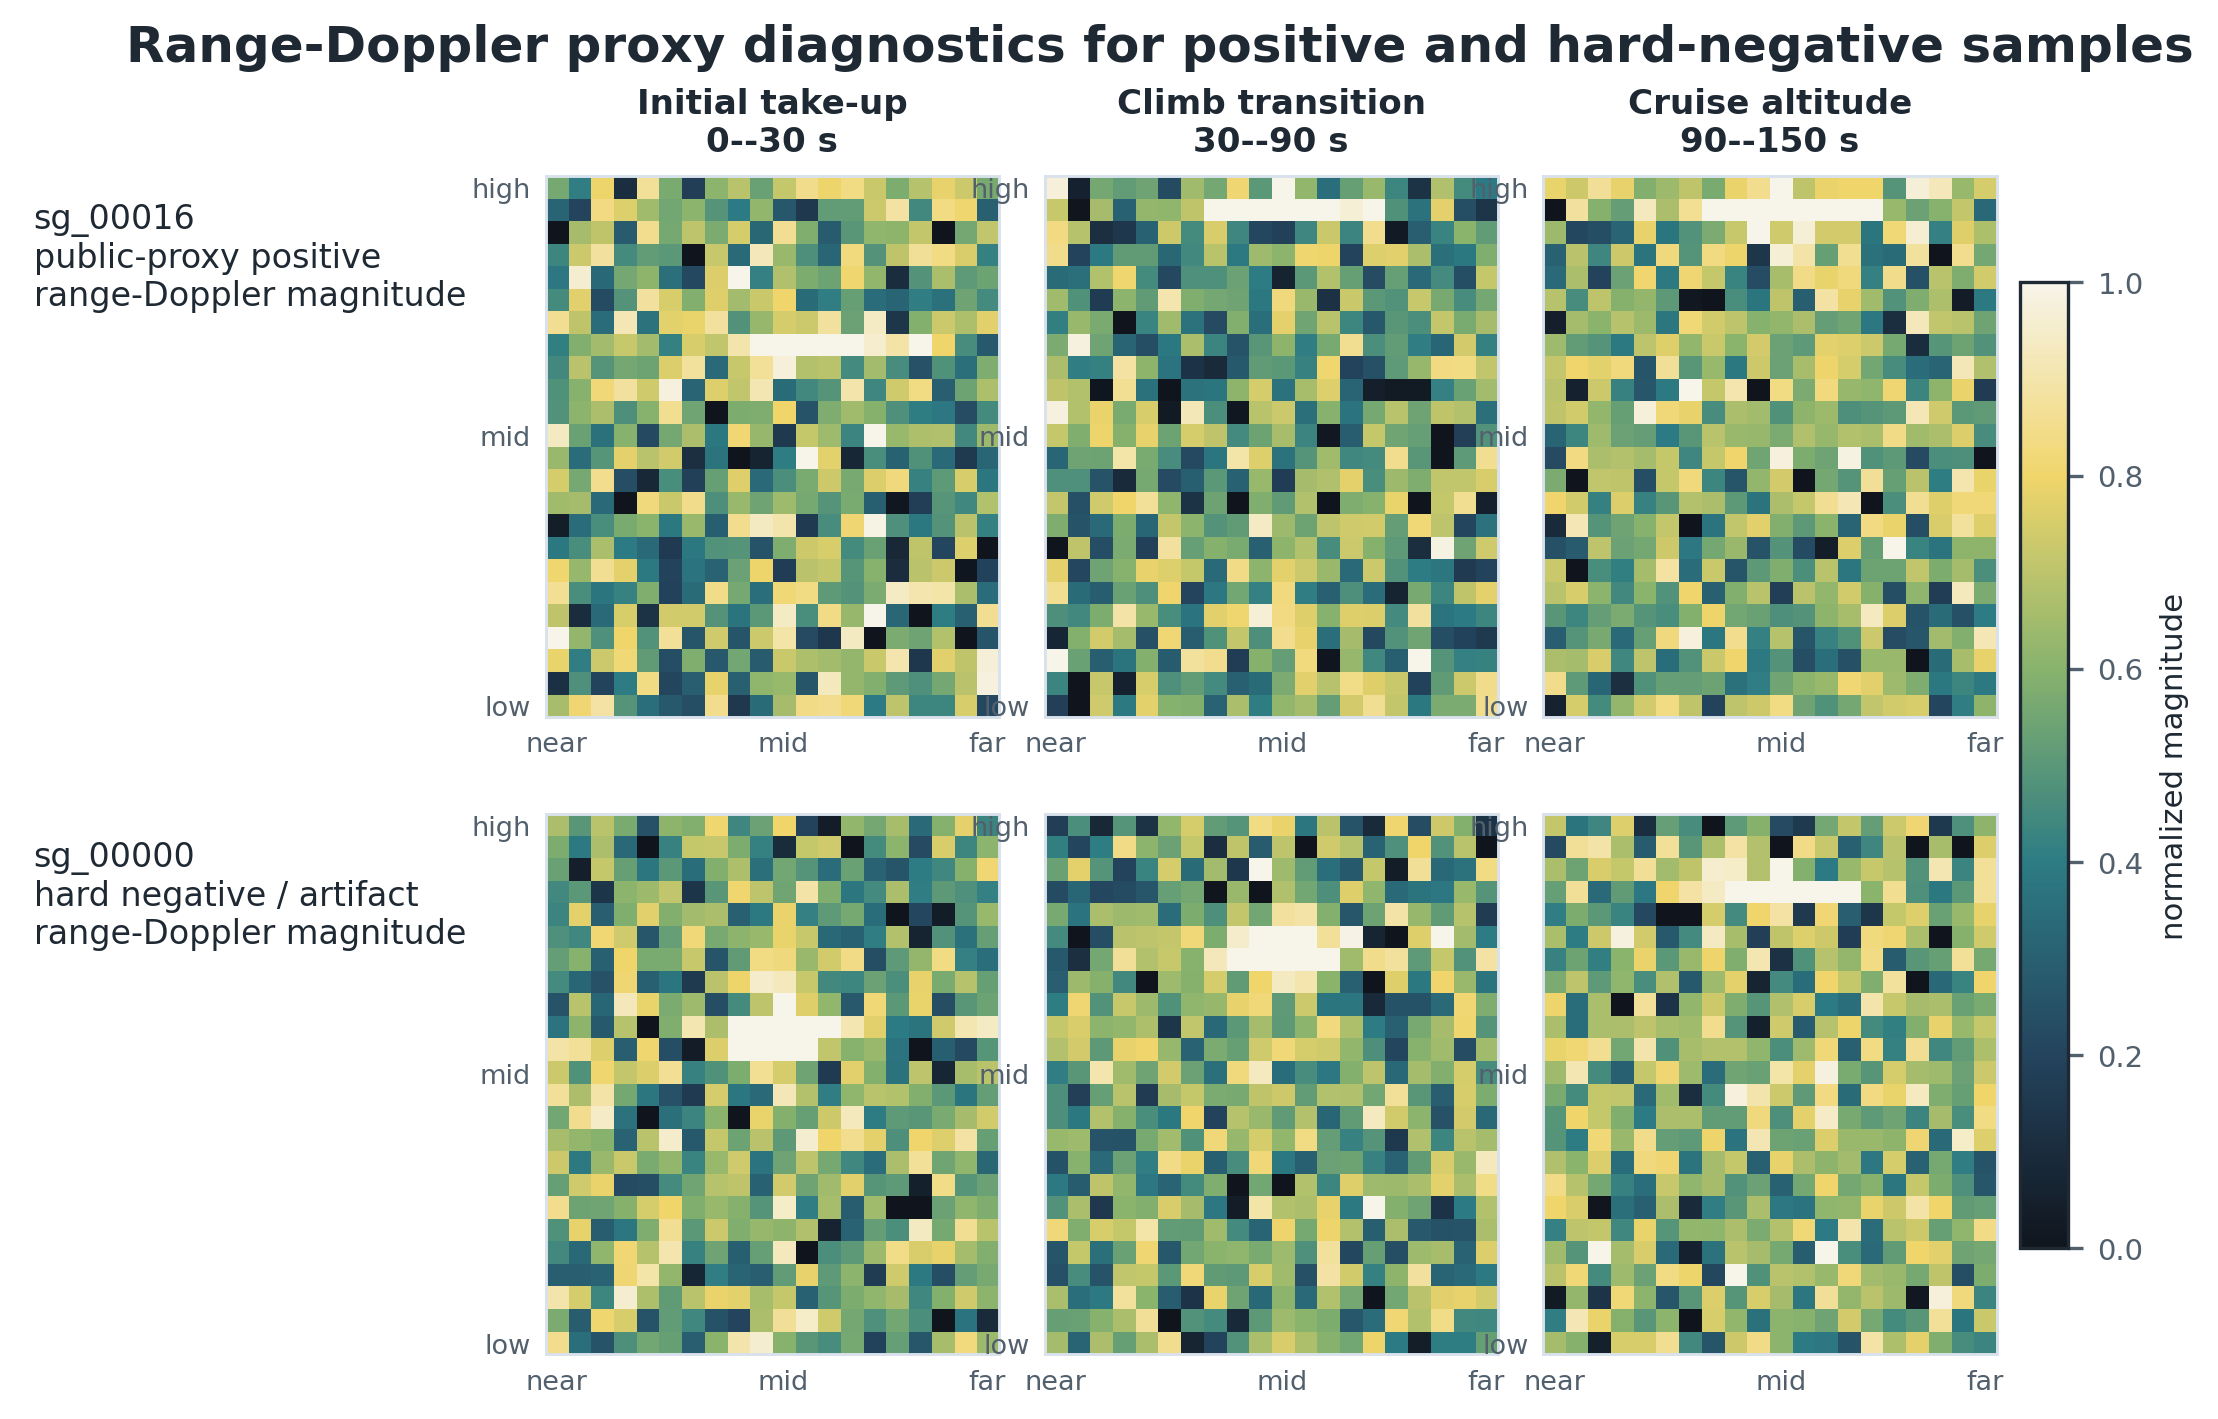
\includegraphics[width=0.98\textwidth]{iq_negative_samples.png}
  \caption{Qualitative range-Doppler proxy sanity panels for a positive public-proxy group and a hard-negative group. Axes show relative range and velocity-equivalent Doppler bins; color is normalized log-magnitude. These panels are qualitative diagnostics, not measured imagery and not detector input for the main KPI.}
  \label{fig:rdpanel}
\end{figure*}

\begin{figure*}[t]
  \centering
  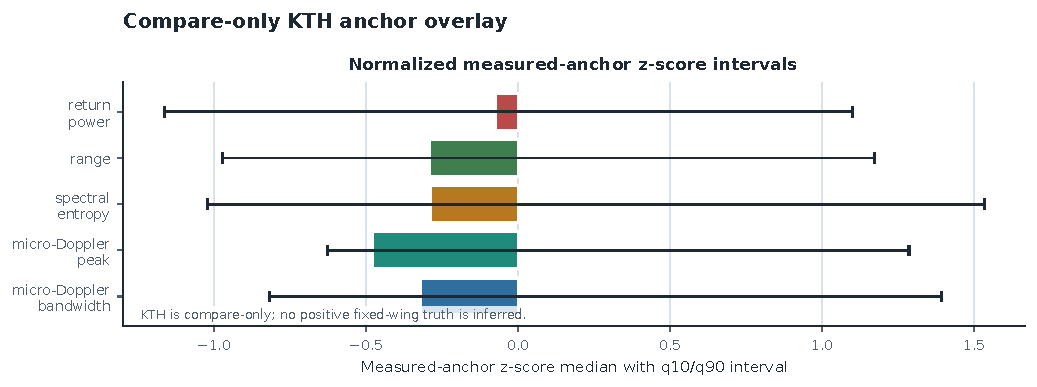
\includegraphics[width=0.98\textwidth]{anchor_overlay.pdf}
  \caption{Compare-only KTH anchor overlay. Features are normalized to measured-anchor z-scores before plotting, so the figure compares distribution shape rather than mixing raw physical units.}
  \label{fig:anchor}
\end{figure*}

The leakage and realism diagnostics include audit-header detection plus model denylisting, label-shuffle sanity, stratum-only and metadata-only baselines, and nearest-neighbor train/holdout scans. The compare-only KTH overlay is useful for distribution-shape checks, not positive-class validation. The comparable view controls also expose a useful critic's point: passive-RF-only ranking can be strong on AP and swept low-FPR recall, but its selected-threshold calibration and lock status differ from the full EI artifact. The paper therefore reports EI as the pre-specified calibrated selected-threshold artifact, not as a universal dominator of every view control.

\section{Limitations}
The most important limitation is also the simplest: a synthetic benchmark is not measured truth. The present corpus should be read as public-proxy evidence with declared priors, not as a fielded sensor surrogate. The comparison against KTH and other public anchors is compare-only and insufficient to justify named-platform claims. That boundary follows the usual verification-and-validation distinction in computational science and reproducibility recommendations for machine-learning research \cite{oberkampf2010,roache1998,peng2011,pineau2021}.

The statistical limitation is central. The corpus is a single-seed run with 50 positive groups total and only eight positive groups in the holdout split. Group-block bootstrap intervals are necessary but not sufficient for broad claims. The physics limitation is also explicit: branch cards use simplified public-proxy RCS, clutter, weather, RFI, waveform, and processing assumptions. The paper contains no hardware-in-the-loop evidence, no measured positive-class validation, no track-level FAR, and no deployment-performance claim. The next useful steps are multi-seed corpora, richer site/weather/RFI stressors, larger positive holdouts, hardware-in-the-loop hooks, and finer-grained uncertainty reporting.

\section{Conclusion}
EchoForge demonstrates a strict-open path for low-altitude UAS radar and multimodal sensing studies: public-proxy priors, deterministic generation, detector-view denylisting, group-locked holdout evaluation, group-block uncertainty estimates, compare-only measured-anchor checks, reproducible detector/fusion benchmarking, and transparent EI-discovered algorithmic improvement. The headline result is LCB95 Recall@$\leq$1\%FPR of 0.713 for EI versus 0.083 for accepted prior fusion, a \kpigain{+760\%} relative gain, with point Recall@$\leq$1\%FPR of 0.833 versus 0.292. These are synthetic public-proxy results under declared assumptions. They are useful for review, robustness work, and reproducible comparison, but they are not measured truth or operational performance claims.

\clearpage
\onecolumn
\appendices

\section{Modeling, Detector, and Source Appendix}
The appendix ledger separates what each source family is used for from what it is not allowed to prove. This is the reviewer-facing boundary for the public-proxy positive class, hard negatives, detector archetypes, and compare-only measured anchors.

\begin{figure}[t]
  \centering
  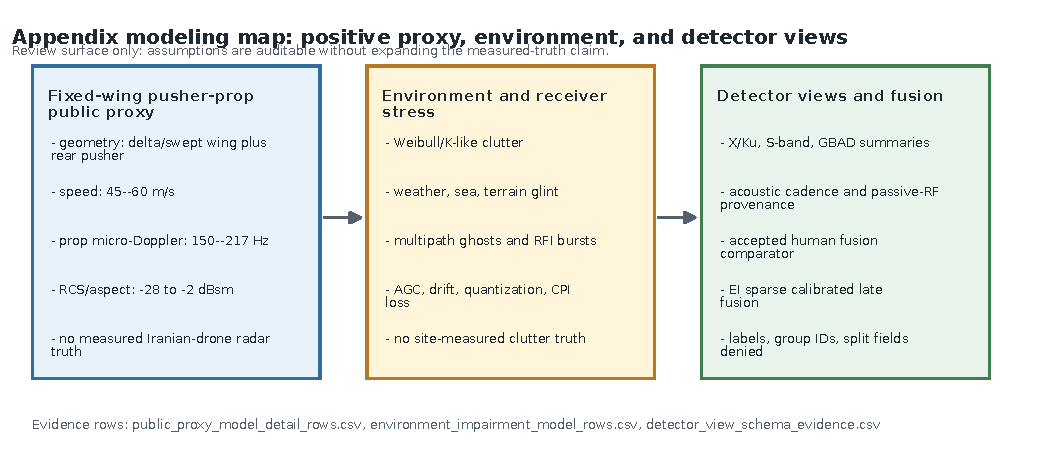
\includegraphics[width=0.98\textwidth]{appendix_modeling_map.pdf}
  \caption{Appendix modeling map for the positive proxy, environment/receiver stress, and detector views. This figure is a review surface: it shows how assumptions are separated from prohibited measured-truth claims.}
  \label{fig:appendixmodelingmap}
\end{figure}

\subsection{Rich Public-Proxy Modeling Appendix}
\label{sec:richmodelappendix}

This appendix states how the benchmark models the positive public-source family, the radar/noise environment, the auxiliary cue families, and hard negatives. The public-source positive class is inspired by open reporting on Iranian fixed-wing pusher-prop loitering-munition families, but EchoForge does \emph{not} claim a measured Iranian-drone radar signature, route model, payload model, or operational performance surrogate. The paper-facing class remains the fixed-wing pusher-prop public proxy.

\begin{table*}[t]
  \caption{Fixed-Wing Pusher-Prop / Iranian-Drone Public-Proxy Modeling Card}
  \label{tab:publicproxymodel}
  \centering
  \small
  \begin{tabular}{@{}p{0.18\textwidth}p{0.25\textwidth}p{0.25\textwidth}p{0.22\textwidth}@{}}
    \toprule
    Modeling item & Public-proxy assumption & Radar consequence & Explicit boundary \\
    \midrule
    Airframe geometry & Delta or swept fixed wing, rear pusher propulsor, approximate 3.3--3.7 m length, 2.3--2.7 m span, 0.35--0.75 m height & Aspect-dependent projected area and RCS envelope & Public visual/summary proxy only; no measured Iranian-platform signature \\
    Launch/take-up & Rail/catapult take-up proxy with short booster-assist stress in the first 0--30 s & Initial phase has ground coupling, multipath, and less settled kinematics & No route, launch-site, operational, or evasion model \\
    Kinematics & 45--60 m/s speed envelope across take-up, climb, and cruise windows & Doppler centroid and track-rate priors for branch summaries & Broad public kinematic envelope only \\
    Propulsion micro-Doppler & Pusher-prop cadence proxy of 150--217 Hz & Narrow high-cadence modulation family distinct from many bird wingbeat bands but overlapping RC prop cadence & Not a measured micro-Doppler signature \\
    RCS/aspect & -28 to -2 dBsm aspect envelope with Swerling-like fluctuation proxy & Controls per-branch detectability and hard-negative overlap & Synthetic stress envelope; no sensor-specific Pd/Pfa claim \\
    Phase labels & Initial take-up 0--30 s, climb transition 30--90 s, cruise altitude 90--150 s & Phase-stratified AP, Recall@$\leq$1\%FPR, and false-alarm diagnostics & Phase conclusions are diagnostic because the holdout has eight positive groups \\
    \bottomrule
  \end{tabular}
\end{table*}

\begin{table*}[t]
  \caption{Noise, Clutter, RFI, and Receiver Modeling Details}
  \label{tab:noisemodeling}
  \centering
  \small
  \begin{tabular}{@{}p{0.18\textwidth}p{0.27\textwidth}p{0.25\textwidth}p{0.20\textwidth}@{}}
    \toprule
    Family & What is generated & Why it matters for radar review & Boundary \\
    \midrule
    Thermal/SNR stress & Synthetic SNR/CNR buckets attached to radar branches and detector-view features & Prevents a trivial clean-signal benchmark & Not a calibrated receiver-noise figure for hardware \\
    Weibull/K-like clutter & Terrain, sea, vegetation, and mixed-scene clutter stressors & Covers non-Gaussian clutter regimes used in radar detection literature & Site-measured clutter truth is not claimed \\
    Weather and sea clutter & Rain/dust/weather-cell, coastal haze, and sea/terrain glint families & Creates near-threshold false-track pressure & Not a meteorological rate model \\
    Multipath ghosts & Synthetic ghost tracks and reflection-like interference & Tests whether fusion overreacts to plausible false tracks & No deployment geometry or site-specific ray tracing \\
    RFI bursts and passive-RF missingness & Sparse RF cues, no-signal behavior, burst contamination, clock-offset, and provenance quality & Tests multimodal fusion when RF is absent, sparse, or contaminated & No emitter library, payload command, operator, or exploitation claim \\
    Receiver impairment & AGC compression, clock drift, quantization, dropped CPI, Doppler folding, and calibration offset & Forces detector views to tolerate sensor-like imperfections & Simplified impairment families, not hardware qualification \\
    \bottomrule
  \end{tabular}
\end{table*}

\begin{table*}[t]
  \caption{Synthetic Radar Simulation Processing Detail}
  \label{tab:radarsimprocessing}
  \centering
  \small
  \begin{tabular}{@{}p{0.16\textwidth}p{0.24\textwidth}p{0.29\textwidth}p{0.21\textwidth}@{}}
    \toprule
    Processing step & Modeled quantity & How it becomes evidence & Red-line boundary \\
    \midrule
    Target return & aspect-dependent public-proxy RCS, phase-stable complex amplitude, range migration, Doppler centroid & IQ magnitude diagnostics and detector features such as concentration and Doppler spread & no measured platform signature \\
    Micro-Doppler & pusher-prop 150--217 Hz proxy plus bird/RC cadence stressors & branch summaries and hard-negative false-alarm interpretation & cadence bands are broad priors, not identity labels \\
    Clutter/noise & thermal/SNR buckets, Weibull/K-like clutter, sea/weather/terrain glint, vegetation motion & score degradation and near-threshold hard-negative pressure & no site-measured clutter truth \\
    Receiver effects & AGC compression, drift, quantization, dropped CPI, Doppler folding, calibration offset & detector-view robustness features and failure slices & no hardware qualification \\
    Cue streams & acoustic cadence/agreement and passive-RF no-signal/RFI/provenance geometry & non-radar branch scores and EI component inputs & no emitter library or operator inference \\
    Feature contract & denylisted schema converts generated products to detector views & train/CV and holdout scores, leakage diagnostics, and KPI tables & labels, split keys, group IDs, and generator internals blocked \\
    \bottomrule
  \end{tabular}
\end{table*}

\begin{table*}[t]
  \caption{Detector-View Modeling Contract}
  \label{tab:detectorviewcontract}
  \centering
  \small
  \begin{tabular}{@{}p{0.16\textwidth}p{0.24\textwidth}p{0.27\textwidth}p{0.23\textwidth}@{}}
    \toprule
    View & Model-facing features & What it can support & What it cannot support \\
    \midrule
    X/Ku radar & Range-Doppler concentration, micro-Doppler spread, CFAR/MTD-style scores, clutter stress & High-resolution radar branch comparison & Proprietary sensitivity, ECCM, or exact vendor Pd/Pfa \\
    S-band radar & Coarser velocity/range summaries, track confidence, multipath stress & Tactical branch stress and cue comparison & Any claimed match to a fielded AESA/MHR implementation \\
    GBAD cueing & Cue confidence, horizon/revisit stress, stale-track state & Wide-area cueing behavior under a public role envelope & Engagement-quality behavior or operator workflow \\
    Acoustic & Spectral cadence, node agreement, weather/traffic stress & Supporting propulsion-cadence cue & Exact microphone layout or field localization performance \\
    Passive RF & No-signal, RFI burst, sparse RF cue, provenance-quality geometry & RF silence/missingness and provenance-quality stress & Emitter identification, command links, payload inference, or operator identity \\
    Fusion & Source confidence, stale-track penalty, cross-sensor confirmation, false-track accounting & Accepted-practice comparator and EI input context & Operational C2 equivalence \\
    \bottomrule
  \end{tabular}
\end{table*}

\begin{table*}[t]
  \caption{Ablation and Appendix Artifact Map}
  \label{tab:appendixartifactmap}
  \centering
  \small
  \begin{tabular}{@{}p{0.22\textwidth}p{0.34\textwidth}p{0.34\textwidth}@{}}
    \toprule
    Artifact & Contents & Reviewer question answered \\
    \midrule
    \texttt{data\_processing\_trace\_rows.csv} & Stage-level scenario-to-holdout trace, including input artifacts, output artifacts, reviewer checks, and claim boundaries & Can I reconstruct the processing path without reading generator internals? \\
    \texttt{main\_kpi\_gain\_table.csv} & Prior-fusion and EI values, absolute changes, relative percentages, and gain/reduction direction & What exactly is the +742\% LCB95 and +185\% point-recall claim computed from? \\
    \texttt{public\_proxy\_model\_detail\_rows.csv} & Positive-class geometry, kinematics, RCS, micro-Doppler, launch, phase, and prohibited-inference rows & How is the Iranian-drone public proxy represented without claiming measured truth? \\
    \texttt{environment\_impairment\_model\_rows.csv} & Clutter, noise, weather, RFI, multipath, receiver impairment, and hard-negative stress rows & What noise and artifact regimes are actually modeled? \\
    \texttt{detector\_view\_schema\_evidence.csv} & Allowed feature families and denied audit-only fields for every detector view & Are labels, split keys, group IDs, or generator state leaking into models? \\
    \texttt{false\_alarm\_by\_method\_family.csv} & Family-wise false alarms for EI and the strongest comparator methods & Which hard negatives generate false alarms and what do the colors in Fig.~\ref{fig:phasekpi} mean? \\
    \texttt{selected\_component\_human\_weights.csv} & Reader-facing EI component weights, modalities, calibrators, and cumulative weights & What does EI fuse at a high level? \\
    \bottomrule
  \end{tabular}
\end{table*}

The appendix is not a claim-expansion device. It is a review surface. It explains the synthetic assumptions behind the benchmark while keeping the central claim narrow: EI improves the low-FPR operating point over accepted fusion practice on this declared synthetic public-proxy run.


\section{Reproducibility CLI Appendix}
These commands reproduce the paper lane; they are benchmark commands, not field-deployment instructions. The generated evidence bundle also emits \texttt{cli\_reproduction\_commands.csv}.

\begin{EchoCodeBox}{Generate the synthetic scenario and sensor corpus}
rtk python3 -m detection.generate_main_run \
  --profile fixed-wing-pusher-proxy-v2 \
  --out-root outputs/training-data/runit-fixed-wing-pusher-proxy-v2-main-run \
  --scenario-groups 10000 \
  --seed 202605210136 \
  --force
\end{EchoCodeBox}

\begin{EchoCodeBox}{Run accepted detector and fusion baselines}
rtk python3 -m detection.run_main_run_detectors \
  --data-root outputs/training-data/runit-fixed-wing-pusher-proxy-v2-main-run \
  --out-root outputs/detection/runit-fixed-wing-pusher-proxy-v2-main-run \
  --folds 5 \
  --seed 202605210136 \
  --force
\end{EchoCodeBox}

\begin{EchoCodeBox}{Run EI search, selection lock, and holdout scoring}
rtk python3 -m detection.run_advanced_main_run_detectors \
  --data-root outputs/training-data/runit-fixed-wing-pusher-proxy-v2-main-run \
  --out-root outputs/detection/runit-fixed-wing-pusher-proxy-v2-main-run-advanced-evolution \
  --folds 5 \
  --seed 202605210136 \
  --search-profile v2_aggressive \
  --candidate-limit 128 \
  --evolution-rounds 5 \
  --evolution-sample-rows 4500 \
  --write-component-scores \
  --force
\end{EchoCodeBox}

\begin{EchoCodeBox}{Build evidence, source appendix, figures, and PDF}
rtk python3 -m detection.paper_evidence --strict-ei-trace --force
rtk python3 paper/generate_source_appendix.py --strict
rtk python3 paper/generate_figures.py --strict
rtk bash paper/build.sh --copy-tracked
rtk python3 paper/validate_paper.py \
  --tex paper/echoforge_ieee.tex \
  --bib paper/references.bib \
  --pdf target/paper/echoforge_ieee.pdf \
  --figures-dir paper/figures \
  --paper-evidence-root outputs/paper-evidence/tier1-final
\end{EchoCodeBox}

\input{target/paper/source_appendix/source_code_appendix.tex}

\bibliographystyle{IEEEtran}
\bibliography{paper/references}

\end{document}
